\documentclass[11pt]{article}

\usepackage[margin=1in]{geometry}
\usepackage{graphicx}
\usepackage{subcaption}
\usepackage{amsmath, amssymb}
\usepackage{booktabs}
\usepackage{hyperref}
\usepackage{xcolor}
\usepackage{float}

\title{\textbf{18-786 HW5: Generating Cat Images with GANs}}
\author{Yizhen Xu \\ Andrew ID: yizhenxu \\ 18-786 Spring 2026}
\date{\today}

\begin{document}
\maketitle

% ==========================================================
\section{Part 1: Deep Convolutional GAN (DCGAN)}

A DCGAN is implemented to generate $64\times 64$ Grumpy-Cat images from the
\texttt{grumpifyBprocessed} dataset (204 images). The generator is built with
\texttt{Upsample}+\texttt{Conv2d} blocks (the first block uses a direct
$4\times 4$ convolution to turn the $1\times 1$ noise into a $4\times 4$ feature
map), and the discriminator is a stack of stride-2 convolutions that compresses
the image down to a single logit. LSGAN-style mean-square loss is used in the
training loop.

\subsection{Training Hyperparameters}
\begin{table}[H]
\centering
\begin{tabular}{ll}
\toprule
Hyperparameter & Value \\
\midrule
Image size & $64\times 64$ \\
Noise size $|z|$ & 100 \\
Base conv width (\texttt{conv\_dim}) & 32 \\
Batch size & 16 \\
Optimizer & Adam ($\beta_1=0.5,\ \beta_2=0.999$) \\
Learning rate & $2\times 10^{-4}$ \\
Loss & LSGAN (mean-squared) \\
Normalization & InstanceNorm \\
Epochs & 500 $\Rightarrow$ $\approx$6{,}500 iterations \\
Sample / checkpoint cadence & every 200 / 400 iter \\
Random seed & 11 \\
\bottomrule
\end{tabular}
\caption{DCGAN training hyperparameters.}
\end{table}

\subsection{Data Augmentation}
Two preprocessing pipelines are compared:
\begin{itemize}
    \item \textbf{Basic:} \texttt{Resize(64)} $\rightarrow$ \texttt{ToTensor} $\rightarrow$ \texttt{Normalize}$(0.5,0.5)$.
    \item \textbf{Advanced:} \texttt{Resize(70)} $\rightarrow$ \texttt{RandomCrop(64)} $\rightarrow$ \texttt{RandomHorizontalFlip} $\rightarrow$ \texttt{ColorJitter}$(0.1,0.1,0.1)$ $\rightarrow$ \texttt{ToTensor} $\rightarrow$ \texttt{Normalize}$(0.5,0.5)$.
\end{itemize}
The advanced pipeline introduces random spatial and photometric perturbations,
which make it much harder for the discriminator to memorize the small training
set.

% ==========================================================
\subsection{Generated Samples}

Figure~\ref{fig:basic-samples} and Figure~\ref{fig:advanced-samples} show
$4\times 4$ sample grids at the beginning (iter 400) and end (iter 6000) of
training for both pipelines. All grids are generated from the same
\emph{fixed} noise batch so that differences reflect the state of the generator
rather than noise variability.

\begin{figure}[H]
    \centering
    \begin{subfigure}[t]{0.45\textwidth}
        \centering
        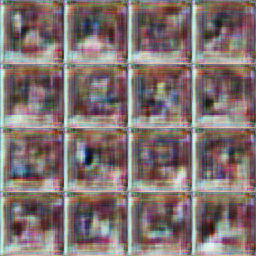
\includegraphics[width=\textwidth]{basic_sample-000400.png}
        \caption{Basic augmentation, iter 400.}
    \end{subfigure}
    \hfill
    \begin{subfigure}[t]{0.45\textwidth}
        \centering
        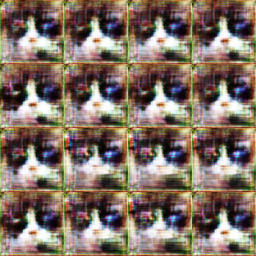
\includegraphics[width=\textwidth]{basic_sample-006000.png}
        \caption{Basic augmentation, iter 6000.}
    \end{subfigure}
    \caption{Generator samples with \textbf{basic} augmentation. At iter 400 the
    output is mostly noise; at iter 6000 the generator has collapsed to nearly
    identical black-and-white cat faces across all 16 grid cells (mode
    collapse).}
    \label{fig:basic-samples}
\end{figure}

\begin{figure}[H]
    \centering
    \begin{subfigure}[t]{0.45\textwidth}
        \centering
        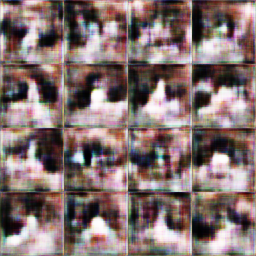
\includegraphics[width=\textwidth]{ad_sample-000400.png}
        \caption{Advanced augmentation, iter 400.}
    \end{subfigure}
    \hfill
    \begin{subfigure}[t]{0.45\textwidth}
        \centering
        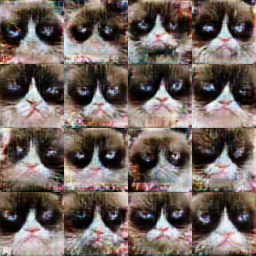
\includegraphics[width=\textwidth]{ad_sample-006000.png}
        \caption{Advanced augmentation, iter 6000.}
    \end{subfigure}
    \caption{Generator samples with \textbf{advanced} augmentation. At iter 400
    the rough positions of the eyes, nose and mouth are already visible. At
    iter 6000 the generator produces clearly recognizable Grumpy-Cat faces with
    distinct ears, eyes and a frowning mouth, and the 16 cells show visibly
    more variation than the basic run (less mode collapse).}
    \label{fig:advanced-samples}
\end{figure}

\paragraph{Visual comparison.}
Advanced augmentation produces images with (i) \emph{less noise} (edges are
sharper, background artifacts are reduced), (ii) \emph{less mode collapse}
(grid cells differ in pose and color), and (iii) \emph{more cat features}
(Grumpy-Cat-specific fur pattern, ears, eyes and nose are clearly rendered).
This matches the ``visually better'' criterion specified in the assignment.

% ==========================================================
\subsection{Training Loss Curves}

Figure~\ref{fig:loss-curves} plots $D_\text{real}$, $D_\text{fake}$ and
$G_\text{loss}$ (log scale on the $y$-axis) for the two runs.

\begin{figure}[H]
    \centering
    \begin{subfigure}[t]{0.48\textwidth}
        \centering
        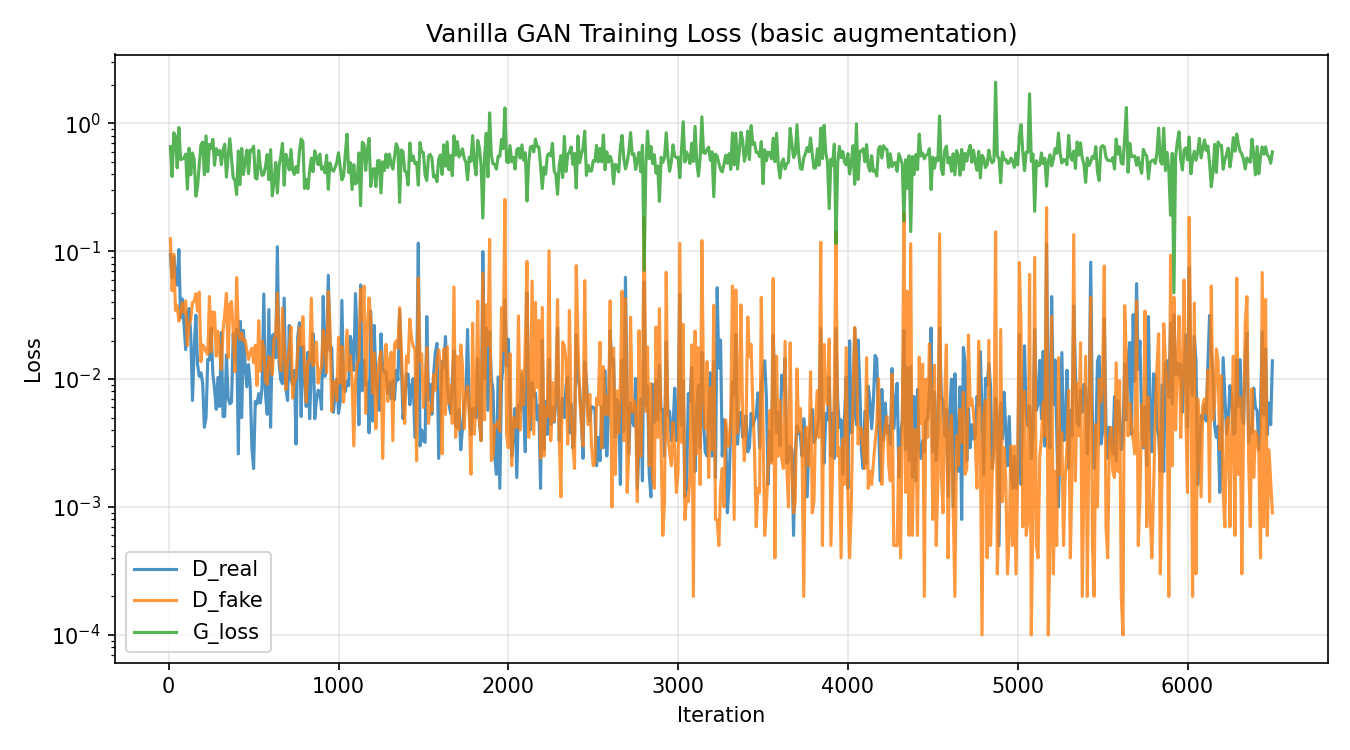
\includegraphics[width=\textwidth]{loss_basic.png}
        \caption{Basic augmentation.}
    \end{subfigure}
    \hfill
    \begin{subfigure}[t]{0.48\textwidth}
        \centering
        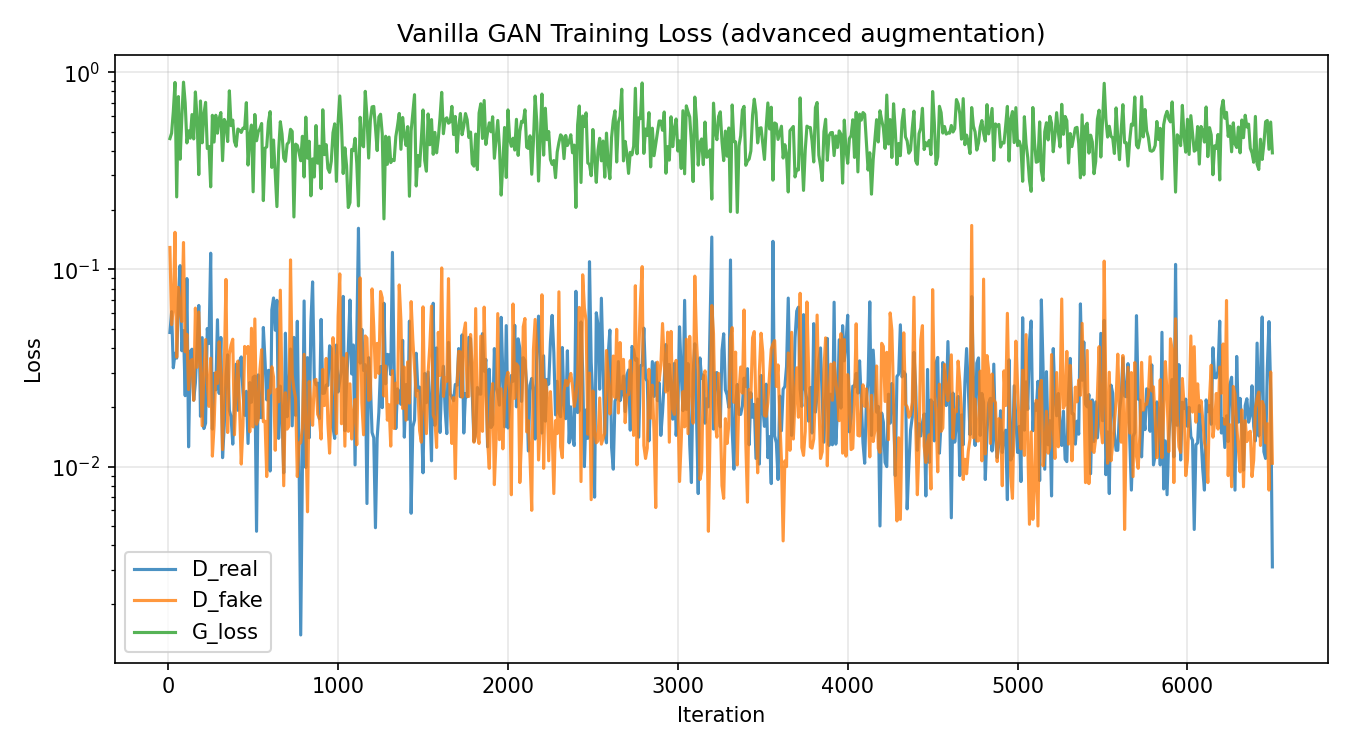
\includegraphics[width=\textwidth]{loss_advanced.png}
        \caption{Advanced augmentation.}
    \end{subfigure}
    \caption{Training loss curves (log-$y$) for the Vanilla-style DCGAN
    (plot script labels it ``Vanilla GAN''; the architecture is the
    DCGAN described in Section~1). The high-frequency oscillation is
    expected — it reflects the adversarial tug-of-war between $G$ and $D$.}
    \label{fig:loss-curves}
\end{figure}

% ==========================================================
\subsection{Analysis}

\paragraph{Oscillation is a healthy signature.}
Unlike supervised training, GANs minimize a min–max objective; every step that
strengthens $D$ forces $G$ to adapt, and vice versa. The losses therefore
oscillate at high frequency throughout training. Neither run shows divergence
(no loss explodes) nor collapse (no loss flatlines at zero), so the adversarial
dynamics themselves are well-behaved.

\paragraph{The key signal: $D_\text{fake}$ behaves differently in the two
runs.}
Table~\ref{tab:dfake} summarizes the order of magnitude of $D_\text{fake}$
through training:

\begin{table}[H]
\centering
\begin{tabular}{lcccc}
\toprule
 & iter 1000 & iter 2000 & iter 4000 & iter 6000 \\
\midrule
$D_\text{fake}$, basic    & 0.021 & 0.003 & 0.0013 & 0.0013 \\
$D_\text{fake}$, advanced & 0.058 & 0.030 & 0.029  & 0.011 \\
\bottomrule
\end{tabular}
\caption{$D_\text{fake}$ at representative iterations (values taken from
\texttt{results/log\_basic.txt} and \texttt{results/log\_advanced.txt}).}
\label{tab:dfake}
\end{table}

In the basic run, $D_\text{fake}$ drops by nearly two orders of magnitude; the
discriminator has effectively memorized the 204 real images and can reject
every fake sample. Once $D$ is nearly perfect, the gradient that flows back to
$G$ vanishes and the generator settles on a single low-variance mode — exactly
the phenomenon observed visually at iter 6000.

In the advanced run, the random crops, flips and color jitter force $D$ to see
a different version of each real image every iteration. $D$ can no longer
memorize and is pushed to learn more generalizable features. $D_\text{fake}$
consequently stays in the $10^{-2}$ range, keeping a non-trivial gradient
flowing into $G$. The generator keeps improving, and mode collapse is avoided.

\paragraph{$G_\text{loss}$ is similar in both runs, and that is expected.}
Under the LSGAN objective $G_\text{loss}=\tfrac12\mathbb{E}[(D(G(z))-1)^2]$
is bounded in $[0, 0.5]$ as long as $D$'s outputs stay in $[0, 1]$. Its
absolute value is a poor indicator of generator quality; what matters is
$D_\text{fake}$ together with the visual samples. Both runs sit around
$G_\text{loss}\approx 0.4\text{--}0.6$, but describe very different
regimes: in basic, $G$ has collapsed to a point that $D$ can trivially reject;
in advanced, $G$ genuinely tracks the real distribution.

\paragraph{Practical heuristics confirmed.}
\begin{itemize}
    \item $D_\text{real}\approx D_\text{fake}\approx 10^{-2}$ with
    $G_\text{loss}\in[0.3,0.7]$ is the healthy equilibrium observed in the
    advanced run.
    \item A joint decay of both $D_\text{real}$ and $D_\text{fake}$ to
    $\leq 10^{-3}$ is an early warning of $D$ overfitting and imminent mode
    collapse, as seen in the basic run.
\end{itemize}

% ==========================================================
\subsection{Conclusion for Part 1}
The DCGAN implementation successfully generates recognizable Grumpy-Cat
images. On the tiny (204-image) training set, basic preprocessing lets the
discriminator overfit, leading to mode collapse after a few thousand
iterations. Advanced data augmentation restores the $G$–$D$ balance: the
generator produces sharper, more diverse and more cat-like samples at iter
6000, while the training losses remain in a healthy oscillating regime.


% ==========================================================
\section{Part 2: Architectures and Objective Functions}

Part 2 compares four GAN variants implemented from scratch (no use of
\texttt{torch.nn.utils.spectral\_norm} or similar wrappers). All four variants
share the same $G$ backbone used in Part 1 (except the custom architecture) and
are trained for $\approx$6{,}500 iterations using the advanced data
augmentation pipeline. The four variants are:
\begin{enumerate}
    \item \textbf{LSGAN} (Mao \emph{et al.}, 2017) — MSE-based objective;
    identical architecture to the DCGAN baseline, only the loss is changed.
    \item \textbf{Spectral Normalization (SN)} (Miyato \emph{et al.}, 2018) —
    power-iteration-based spectral normalization applied to every convolution
    in the discriminator, turning $D$ into a 1-Lipschitz network.
    \item \textbf{WGAN-GP} (Arjovsky 2017, Gulrajani 2017) — the discriminator
    becomes a critic with a real-valued score; the loss is the Wasserstein-1
    dual plus a gradient penalty $\lambda\,\mathbb{E}[(\|\nabla_{\hat x}
    D(\hat x)\|_2 - 1)^2]$ on random interpolations $\hat x=\varepsilon
    x+(1-\varepsilon)G(z)$. The critic is updated $n_\text{critic}{=}5$ times
    per generator step; Adam uses $\beta_1{=}0.0,\beta_2{=}0.9$.
    \item \textbf{Custom} — a residual, spectrally-normalized architecture:
    \texttt{ResnetBlock}s are inserted after each upsample in $G$, and the
    discriminator uses SN on every convolution plus two SN \texttt{ResBlock}s
    at intermediate resolutions. Trained with the LSGAN objective.
\end{enumerate}

\subsection{Training Hyperparameters (Part 2)}
\begin{table}[H]
\centering
\begin{tabular}{lcccc}
\toprule
 & LSGAN & SN & WGAN-GP & Custom \\
\midrule
Loss     & MSE & MSE & Wasserstein + GP & MSE \\
Adam $(\beta_1,\beta_2)$ & $(0.5,0.999)$ & $(0.5,0.999)$ & $(0.0,0.9)$ & $(0.5,0.999)$ \\
$n_\text{critic}$ & 1 & 1 & 5 & 1 \\
$\lambda_\text{GP}$ & — & — & 10 & — \\
Norm in $D$ & InstanceNorm & none (SN only) & LayerNorm (GN$_1$)\footnotemark & none (SN only) \\
\bottomrule
\end{tabular}
\caption{Part 2 variant-specific hyperparameters. Image size, noise size,
batch size, learning rate and total iterations are the same as Part 1.}
\end{table}
\footnotetext{GN$_1$ denotes \texttt{GroupNorm(num\_groups=1, C)}, which is
mathematically equivalent to per-sample \texttt{LayerNorm} over the spatial
dimensions. This is the normalization recommended by the WGAN-GP paper, since
BatchNorm breaks the per-sample gradient penalty.}

% ==========================================================
\subsection{Generated Samples at Iteration 6000}

Figure~\ref{fig:part2-samples} shows the $4\times 4$ sample grids produced by
each variant at the end of training, all generated from the same fixed noise
batch.

\begin{figure}[H]
    \centering
    \begin{subfigure}[t]{0.24\textwidth}
        \centering
        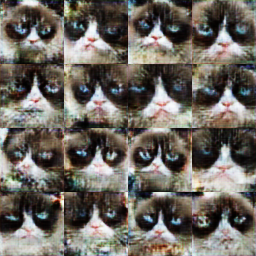
\includegraphics[width=\textwidth]{lsgan_sample-006000.png}
        \caption{LSGAN.}
    \end{subfigure}
    \hfill
    \begin{subfigure}[t]{0.24\textwidth}
        \centering
        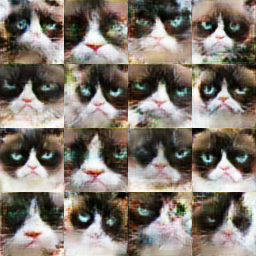
\includegraphics[width=\textwidth]{sn_sample-006000.png}
        \caption{Spectral Norm.}
    \end{subfigure}
    \hfill
    \begin{subfigure}[t]{0.24\textwidth}
        \centering
        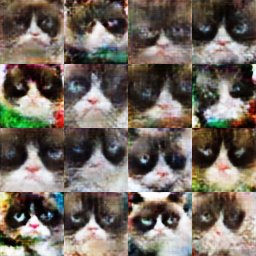
\includegraphics[width=\textwidth]{wgangp_sample-006000.png}
        \caption{WGAN-GP.}
    \end{subfigure}
    \hfill
    \begin{subfigure}[t]{0.24\textwidth}
        \centering
        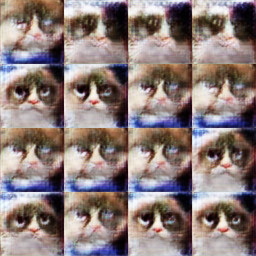
\includegraphics[width=\textwidth]{custom_sample-006000.png}
        \caption{Custom.}
    \end{subfigure}
    \caption{Generator samples at iter 6000 for the four Part 2 variants
    (fixed noise). LSGAN and SN produce recognizable faces with mild
    background artifacts; WGAN-GP shows stronger texture noise; the Custom
    architecture yields the sharpest, cleanest results with clearly rendered
    white chest fur, chin, frowning mouth and ear shape.}
    \label{fig:part2-samples}
\end{figure}

% ==========================================================
\subsection{Training Loss Curves}

Figures~\ref{fig:part2-loss-each}–\ref{fig:part2-loss-wgan} show the training
losses for each variant. The LSGAN-style variants (LSGAN, SN, Custom) share
the same loss axes; WGAN-GP is plotted separately because its loss is an
unbounded real-valued Wasserstein estimate and additionally provides two
diagnostic quantities (the estimated Wasserstein distance and the gradient
penalty).

\begin{figure}[H]
    \centering
    \begin{subfigure}[t]{0.48\textwidth}
        \centering
        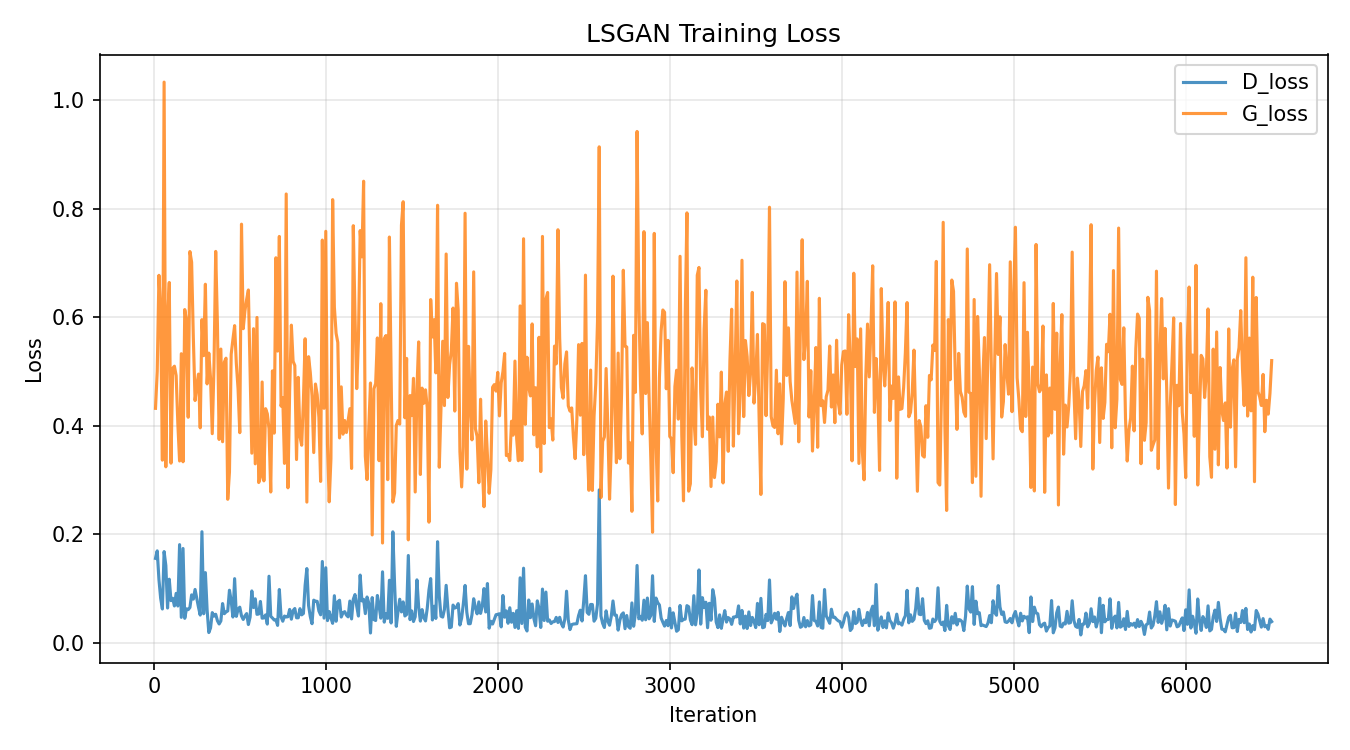
\includegraphics[width=\textwidth]{loss_lsgan.png}
        \caption{LSGAN.}
    \end{subfigure}
    \hfill
    \begin{subfigure}[t]{0.48\textwidth}
        \centering
        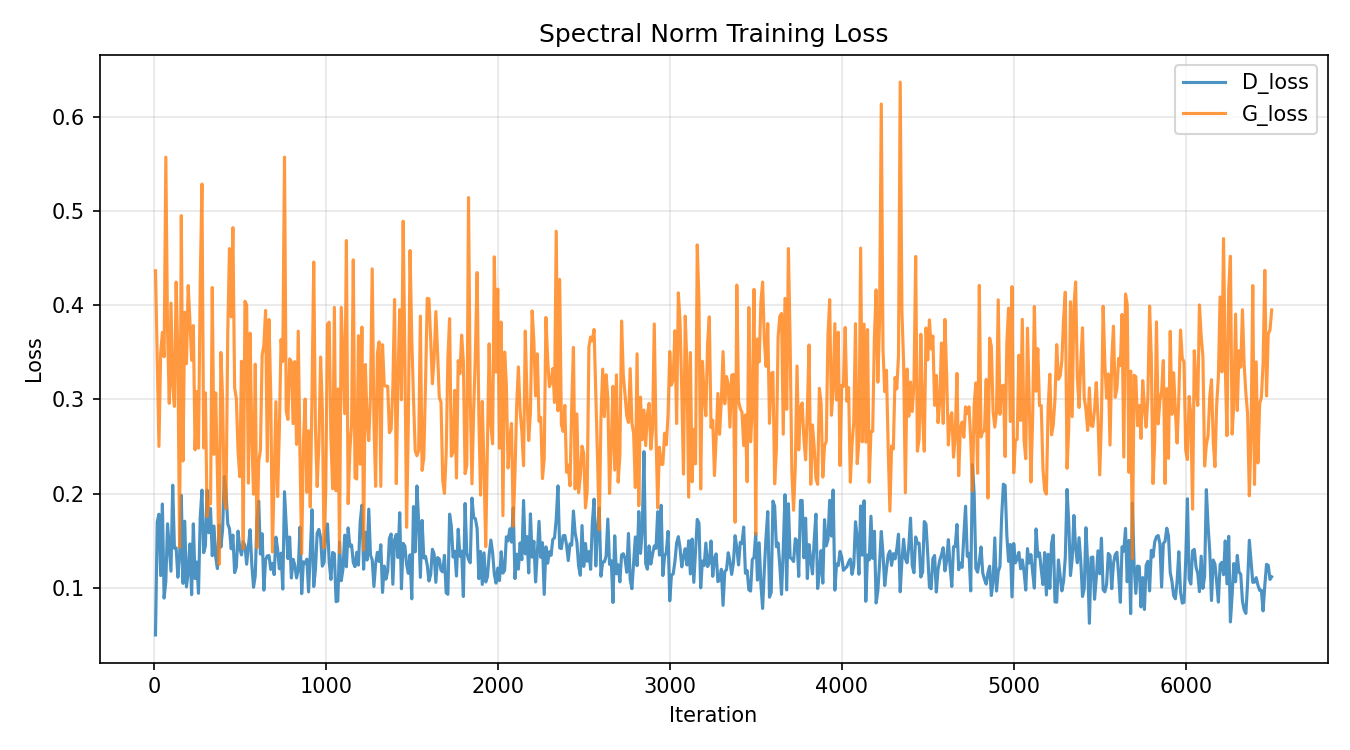
\includegraphics[width=\textwidth]{loss_sn.png}
        \caption{Spectral Norm.}
    \end{subfigure}

    \vspace{0.5em}

    \begin{subfigure}[t]{0.48\textwidth}
        \centering
        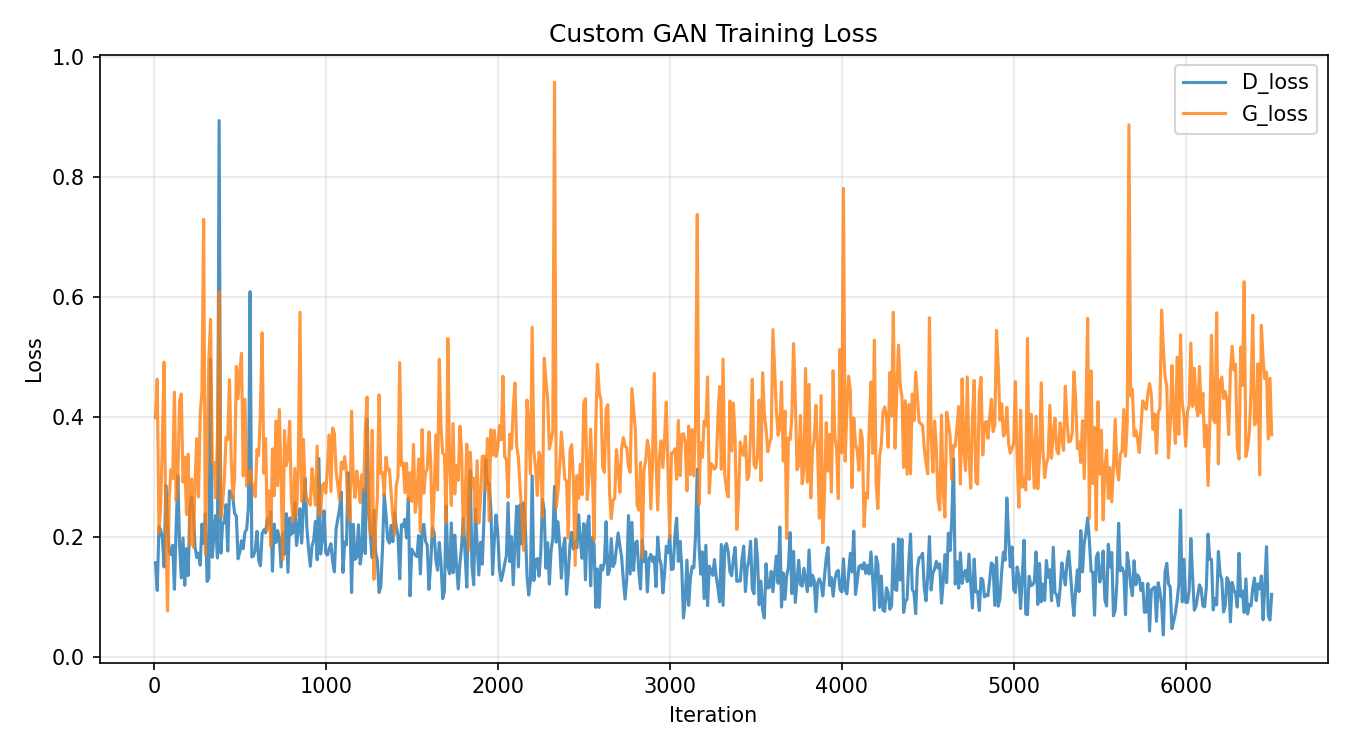
\includegraphics[width=\textwidth]{loss_custom.png}
        \caption{Custom.}
    \end{subfigure}
    \caption{LSGAN-style variants: $D_\text{loss}$ and $G_\text{loss}$
    throughout training. Enlarged for readability; WGAN-GP is plotted
    separately in Figure~\ref{fig:part2-loss-wgan} because its loss sits
    on a different (signed, unbounded) scale.}
    \label{fig:part2-loss-each}
\end{figure}

\begin{figure}[H]
    \centering
    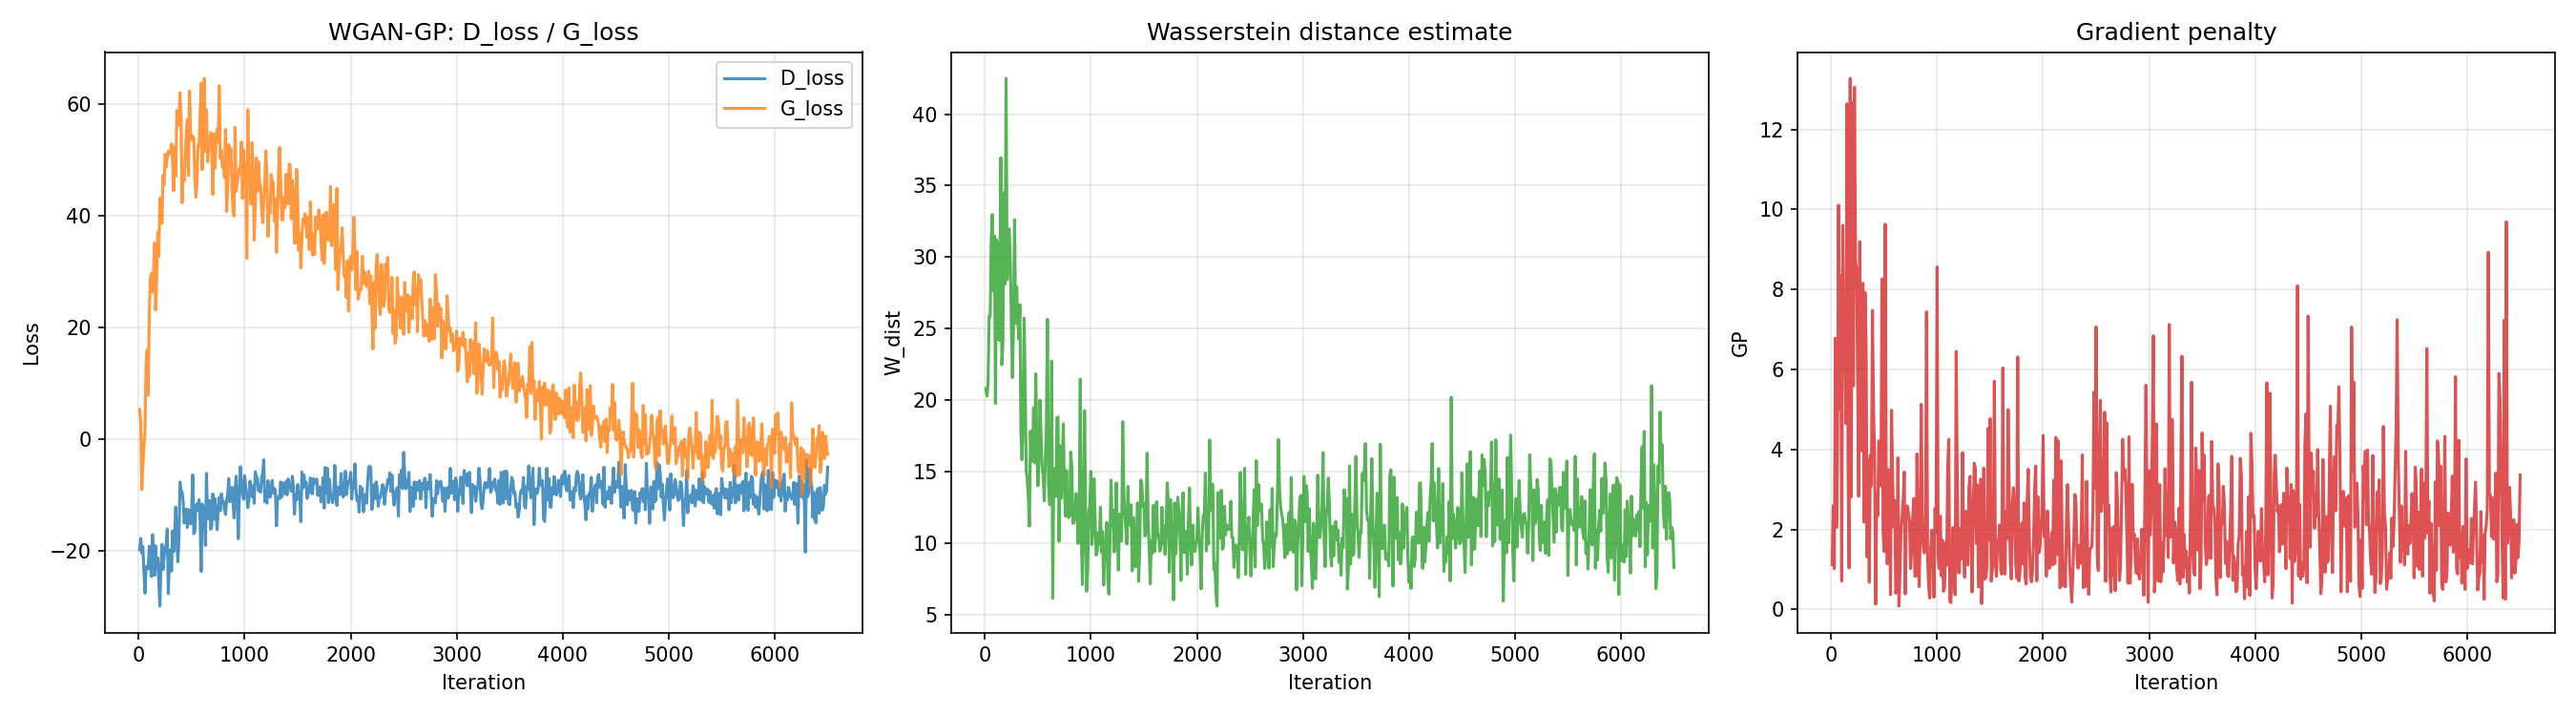
\includegraphics[width=\textwidth]{loss_wgan_gp.png}
    \caption{WGAN-GP diagnostics: (left) $D_\text{loss}$ and $G_\text{loss}$,
    (middle) the Wasserstein distance estimate
    $\hat W = \mathbb{E}[D(\text{real})]-\mathbb{E}[D(\text{fake})]$, (right)
    the gradient penalty term.}
    \label{fig:part2-loss-wgan}
\end{figure}

% ==========================================================
\subsection{Analysis}

\paragraph{$D_\text{loss}$ magnitudes reveal which variant best balances
$G$ and $D$.}
Averaging over the second half of training, the MSE-based variants settle at
\begin{itemize}
    \item LSGAN: $D_\text{loss}\approx 0.04$, $G_\text{loss}\approx 0.45$.
    \item Spectral Norm: $D_\text{loss}\approx 0.10$, $G_\text{loss}\approx 0.38$.
    \item Custom: $D_\text{loss}\approx 0.10$, $G_\text{loss}\approx 0.40$.
\end{itemize}
The discriminator loss under SN and Custom is \emph{2–3$\times$ larger} than
under plain LSGAN. This is exactly the effect predicted by the SN paper: the
1-Lipschitz constraint prevents $D$ from becoming arbitrarily confident, which
keeps a non-trivial gradient flowing into $G$. Consistent with this, the
generator loss is slightly \emph{lower} for SN/Custom: because the
Lipschitz-bounded discriminator has limited expressive power (output values
cannot grow arbitrarily far from each other across inputs), the same generator
can reach a higher $D(G(z))$ score — not because $G$ is qualitatively better,
but because $D$ is constrained to be smoother.

\paragraph{Stability ranking.}
Because WGAN-GP uses a signed, unbounded Wasserstein loss whereas the other
three use bounded MSE losses in $[0,1]$, it is not meaningful to compare their
oscillation amplitudes directly. The ranking is therefore given in two
groups.

\smallskip
\noindent\textit{Among the MSE-based variants} (smoothest first):
\begin{enumerate}
    \item \textbf{Spectral Norm} — cleanest, smallest-amplitude oscillation.
    \item \textbf{LSGAN} — healthy but noisier peaks up to $G\!\approx\!1.0$.
    \item \textbf{Custom} — SN-level baseline with occasional spikes to
    $\approx\!0.9$; these are caused by the additional ResBlock depth but
    decay quickly and never cause divergence.
\end{enumerate}

\noindent\textit{WGAN-GP} is evaluated on its own terms (see next paragraph):
its raw $D_\text{loss}$ spans tens of units and cannot be put on the same
axes, but the Wasserstein-distance estimate $\hat W$ and the gradient-penalty
term give direct diagnostics of stability.

\paragraph{WGAN-GP: what the three diagnostic panels mean.}
\begin{itemize}
    \item The \emph{left} panel shows $G_\text{loss}$ (orange) descending from
    roughly $+60$ toward $0$ during the first 4{,}000 iterations. Unlike the
    MSE variants where $G_\text{loss}$ only oscillates, the WGAN generator
    loss is directly proportional to $-\mathbb{E}[D(G(z))]$; its monotone
    decrease is a meaningful signal that the critic increasingly accepts the
    generator's samples.
    \item The \emph{middle} panel plots the Wasserstein distance estimate.
    Ideally this should decrease monotonically toward a small constant. It
    decreases from $\approx\!40$ to the range $[8,13]$ but is still
    oscillating at iter 6{,}500 — the model is \emph{not fully converged} yet.
    This is consistent with the small training set (204 images) and the fact
    that, with $n_\text{critic}{=}5$, the generator has only performed
    $\approx\!1{,}300$ update steps.
    \item The \emph{right} panel plots the gradient penalty. It falls from
    $\approx\!12$ to the range $[1,5]$, showing that the 1-Lipschitz
    constraint is approximately, but not perfectly, satisfied.
\end{itemize}
The visual samples are therefore coarser than those of SN / Custom, and this
under-training is the likely cause — not a flaw in the WGAN-GP method itself.

\paragraph{Custom wins visually despite noisier losses.}
The Custom architecture exhibits more loss spikes than SN, yet produces the
sharpest samples of all four variants. This is a useful reminder that
loss-curve smoothness and sample quality are \emph{not} the same thing: the
deeper residual $G$ makes optimization bumpier in exchange for a richer
function class. In this experiment the trade-off is favorable.

% ==========================================================
\subsection{Conclusion for Part 2}
All four variants produce recognizable Grumpy-Cat images with the advanced
augmentation pipeline. Spectral normalization demonstrably stabilizes training
(smoother losses, higher equilibrium $D_\text{loss}$) without harming quality.
The Custom architecture — combining spectral normalization with residual
blocks in both $G$ and $D$ — yields the best visual quality, confirming that
architectural improvements compound with stabilization techniques. WGAN-GP
produces meaningful but visibly undertrained samples within the 6{,}500
iterations budget; its descending $G_\text{loss}$ and shrinking gradient
penalty suggest that longer training would close the gap.

\paragraph{Final visual-quality ranking.}
Considering sharpness, absence of background artifacts and the correct
rendering of cat-specific features (chest fur, ears, frowning mouth), the
end-of-training samples rank as
\[
\text{Custom} \;>\; \text{SN} \;\approx\; \text{LSGAN} \;>\; \text{WGAN-GP},
\]
with the caveat that WGAN-GP's last-place finish reflects under-training
rather than an intrinsic weakness of the objective.

% ==========================================================
\begin{thebibliography}{9}

\bibitem{goodfellow2014gan}
I. J. Goodfellow, J. Pouget-Abadie, M. Mirza, B. Xu, D. Warde-Farley, S. Ozair,
A. Courville, and Y. Bengio.
\newblock Generative adversarial nets.
\newblock In \emph{NeurIPS}, 2014.

\bibitem{radford2016dcgan}
A. Radford, L. Metz, and S. Chintala.
\newblock Unsupervised representation learning with deep convolutional
generative adversarial networks.
\newblock In \emph{ICLR}, 2016.

\bibitem{mao2017lsgan}
X. Mao, Q. Li, H. Xie, R. Y. K. Lau, Z. Wang, and S. P. Smolley.
\newblock Least squares generative adversarial networks.
\newblock In \emph{ICCV}, 2017.

\bibitem{arjovsky2017wgan}
M. Arjovsky, S. Chintala, and L. Bottou.
\newblock Wasserstein generative adversarial networks.
\newblock In \emph{ICML}, 2017.

\bibitem{gulrajani2017wgangp}
I. Gulrajani, F. Ahmed, M. Arjovsky, V. Dumoulin, and A. C. Courville.
\newblock Improved training of Wasserstein GANs.
\newblock In \emph{NeurIPS}, 2017.

\bibitem{miyato2018sn}
T. Miyato, T. Kataoka, M. Koyama, and Y. Yoshida.
\newblock Spectral normalization for generative adversarial networks.
\newblock In \emph{ICLR}, 2018.

\end{thebibliography}


\end{document}
